% !TEX program = pdflatex
\documentclass[10pt,a4paper]{article}
\usepackage[T1]{fontenc}
\usepackage[utf8]{inputenc}
\usepackage{lmodern}
\usepackage[margin=2cm]{geometry}
\usepackage{amsmath,amssymb}
\usepackage{graphicx}
\usepackage{booktabs}
\usepackage{array}
\usepackage{tabularx}
\usepackage{float}
\usepackage{caption}
\usepackage[hidelinks]{hyperref}
\newcolumntype{Y}{>{\centering\arraybackslash}X}
\captionsetup{font=small,labelfont=bf}
\setlength{\parindent}{0pt}
\setlength{\parskip}{3.5pt}
\graphicspath{{./}{./output/figures/}{./output/plots/}}
\title{SSVI Implied-Volatility Surface Dynamics \& Realized-Volatility Forecasting \\[2pt] \large Evidence from S\&P 500 Options (2010--2020)}
\author{Alessio Porrini, Marco Amarilli, Camilla Introzzi, Christian Frigerio}
\date{Econometrics Project --- Academic Year 2025/26 \\ Politecnico di Milano --- Insurance \& Econometrics}
\begin{document}
\maketitle
\vspace{-1.2em}
\begin{abstract}\noindent Using $\sim$1.5 million filtered S\&P 500 option quotes (2010--2020), we calibrate a daily arbitrage-free SSVI implied-volatility surface and ask whether its structural information improves the modelling and forecasting of its own parameters and of realized volatility (RV), relative to random-walk and HAR benchmarks. The central result is \textit{negative with informational content}: a single asset's own option surface does not beat a parsimonious HAR for RV forecasting through the COVID-19 window, and the surface behaves as a near-efficiently-priced object at the daily frequency. We exercise the full course toolbox --- panel regression with fixed/random effects and hypothesis testing, ARMA/ARMAX, VAR, non-stationarity and cointegration, and point/probabilistic forecasting --- and add two original contributions: a deliberately asset-agnostic (VIX-free) RV-forecasting study (Notebook C) and an Avellaneda \& Stoikov (2008) surface market-making risk engine with an SSVI-based, ES\textsubscript{95}-calibrated residual add-on (Notebook D). \end{abstract}


\section*{1. Introduction and Literature Review}

\textbf{Research aims.} The project pursues two connected research questions:

\begin{itemize}\setlength{\itemsep}{1pt}
\item \textbf{RQ1 --- Predictive content / market efficiency.} Does the structural information in an arbitrage-free IV surface carry incremental out-of-sample (OOS) predictive content for (a) its own future dynamics and (b) future realized volatility, beyond simple benchmarks (random walk, HAR)? A sharpened, deliberately asset-agnostic version asks whether a single underlying's \textit{own} option surface can supply the regime information usually drawn from the VIX --- specific to the S\&P 500 --- in a form portable to any asset with a liquid option market.
\item \textbf{RQ2 --- Risk-management application.} Can the \textbf{Avellaneda \& Stoikov (2008)} optimal market-making framework, which sets quotes for a single instrument, be extended to the full implied-volatility surface with an SSVI-based residual-risk add-on calibrated to a target tail (Expected-Shortfall) coverage?
\end{itemize}

The first is the efficient-pricing question; the second turns the surface model into a deployable quoting-and-risk tool.

\textbf{Economic framework.} Under efficient option pricing the no-arbitrage IV surface should be close to a martingale at short horizons: if daily surface increments were systematically predictable, a delta-hedged position would extract near risk-free profit, which a functioning market arbitrages away. The competing hypothesis --- from the long-memory and path-dependence literature --- is that volatility (realized \textit{and} implied) carries persistent, multi-horizon structure that low-order autoregressive models miss but a long-memory model can exploit.

\textbf{Literature.} The methodological backbone rests on three works. We parametrise the surface with the SSVI model of \textbf{Gatheral \& Jacquier (2014)}, which guarantees freedom from static (butterfly and calendar) arbitrage. The forecasting backbone is the Heterogeneous Autoregressive (HAR) model of \textbf{Corsi (2009)}, which approximates the long memory of realized volatility --- documented by \textbf{Andersen, Bollerslev, Diebold \& Labys (2003)} --- with cascaded daily/weekly/monthly components. The hypothesis that the IV surface is itself \textit{path-dependent}, and hence amenable to HAR-type modelling, is the recent contribution of \textbf{Andr\`{e}s, Boumezoued \& Jourdain (2025)}, which directly motivates applying HAR to the SSVI parameters. For the risk engine we build on \textbf{Avellaneda \& Stoikov (2008)}. Supporting tools: \textbf{Johansen (1991)} and \textbf{Engle \& Granger (1987)} for cointegration, \textbf{Bollerslev (1986)} GARCH for conditional heteroskedasticity, and the \textbf{Diebold \& Mariano (1995)} test (small-sample corrected) for formal forecast comparison.

\section*{2. Data and Methodology}

\subsection*{2.1 Dataset (primary focus)}

\textbf{Source and composition.} The raw dataset is a panel of daily \textbf{S\&P 500 European option} quotes spanning 2010-01-01 $\rightarrow$ 2020-12-31 ($\sim$2,769 trading files; $\sim$3.33 million raw rows), each carrying strike, option type, bid/ask/mid, open interest and time-to-expiry (TTE). Zero-coupon \textbf{Treasury rates} (1M, 3M, 6M, 1Y, 2Y, 3Y) and the \textbf{VIX} are pulled from FRED; the SPX spot is from Yahoo Finance. The data are processed in three notebooks (\texttt{00\_data\_preparation}, \texttt{01\_iv\_dataset\_construction}, \texttt{02\_ssvi\_calibration}).

\textbf{Cleaning pipeline (core technique \#1).} Quality filters remove illiquid and economically meaningless quotes --- mid price $>$ \$0.05, time-to-expiry $>$ 7 days, relative bid-ask spread $\le$ 30\%, and log-moneyness $\in$ [-0.40, 0.30]. The implied \textbf{forward} is extracted per maturity via put-call parity; Black-76 \textbf{implied volatility} is then computed by vectorised Newton-Raphson. At the calibration stage we apply a further \textbf{maturity-dependent delta filter}: far-OTM quotes whose absolute Black-Scholes delta falls below a band tightening from 0.30 at the shortest maturities to 0.05 at the longest ($\Delta_{\min}(T) = 0.05 + 0.25\,e^{-3T}$) are discarded, removing illiquid wings and keeping OTM puts and calls balanced before the arbitrage-free fit. The funnel is:

\begin{center}\small
\begin{tabular}{ll}
\toprule
\textbf{Stage} & \textbf{Count} \\
\midrule
Raw rows & $\sim$3,331,302 \\
After domain/liquidity filters & $\sim$2,324,008 \\
Black-76 IV retained & $\sim$1,500,012 \\
SSVI calibration success & 2,633 / 2,768 days (\textbf{95.1\%}) \\
\bottomrule
\end{tabular}
\end{center}

\textbf{Derived parameter panel.} For each trading day we calibrate the SSVI surface, yielding a daily time series of the five parameters ($\alpha$, $\beta$, $\rho$, $\eta$, $\gamma$). Calibration succeeds on \textbf{95.1\%} of days with median RMSE\_iv $<$ 0.01 and \textbf{zero} calendar-arbitrage violations --- this calibrated panel is the input to all downstream time-series analysis (Notebooks B and D). The realized-volatility target (Notebook C) is a daily log-RV proxy built from SPX returns.

\subsection*{2.2 SSVI parametrisation and parameter economics}

$$\omega(k,\theta) = \frac{\theta}{2}\left\{1 + \rho\,\phi(\theta)\,k + \sqrt{(\phi(\theta)\,k+\rho)^2 + (1-\rho^2)}\right\}, \quad \phi(\theta) = \frac{\eta\,\theta^{-\gamma}}{1+\eta\,\theta^{1-\gamma}}$$

The five calibrated parameters carry direct economic readings (sample means in parentheses): \textbf{$\alpha$} = log ATM variance / surface level (-3.45), \textbf{$\beta$} = term-structure slope (1.19), \textbf{$\rho$} = skew / leverage effect (-0.77), \textbf{$\eta$} = vol-of-vol / smile width (0.75), \textbf{$\gamma$} = term-structure decay rate (0.54).

\subsection*{2.3 Econometric toolbox --- coverage of the core techniques}

The project applies every core econometric technique of the course to the volatility data; the table maps each to its implementation. Section 3 mirrors this mapping, giving each method a self-contained results subsection (\S{}3.1--\S{}3.5), followed by the two original contributions (\S{}3.6).

\begin{center}\footnotesize
\begin{tabularx}{\textwidth}{@{}c >{\raggedright\arraybackslash}p{3.0cm} X >{\raggedright\arraybackslash}p{1.6cm}@{}}
\toprule
\textbf{\#} & \textbf{Core technique} & \textbf{Implementation} & \textbf{Reported in} \\
\midrule
1 & Data cleaning, trend \& seasonality & Cleaning funnel (NB 00--02); trend via I(d) classification + differencing; seasonality assessed and justified immaterial & \S{}2.1, \S{}3.1 \\
2 & Linear regression + hypothesis testing & Panel IV regression with t/F-tests, RESET (NB A); OLS feature-significance pruning (NB C) & \S{}3.2 \\
3 & Fixed \& random effects & Pooled OLS $\rightarrow$ Day FE $\rightarrow$ Day$\times$Maturity FE $\rightarrow$ Surface-Cell FE, \textbf{Hausman test} FE-vs-RE (NB A) & \S{}3.2 \\
4 & ARMA models & BIC-optimal ARMA + \textbf{ARMAX} (exogenous VIX) on 10 series (NB B) & \S{}3.4 \\
5 & Point \& probabilistic forecasting & Multi-horizon RV point forecasts + DM (NB C); \textbf{AR-GARCH 80\% prediction intervals} (NB B); \textbf{ES\textsubscript{95} coverage} (NB D) & \S{}3.5 \\
6 & VAR models & VAR(2, BIC) on the 5-parameter system + \textbf{VECM} (NB B) & \S{}3.4 \\
7 & Non-stationarity \& cointegration & ADF + KPSS, \textbf{Johansen} trace, \textbf{Engle-Granger}, rolling Johansen (NB B) & \S{}3.3 \\
\bottomrule
\end{tabularx}
\end{center}

\textbf{Evaluation metrics.} OOS skill is measured by $R^2_\text{OOS} = 1 - \sum_t (y_t-\hat y_t)^2 / \sum_t (y_t-y_{t-1})^2$ (relative to the na\"{\i}ve random-walk benchmark, so $R^2_\text{OOS}=0$ for the na\"{\i}ve model by construction), and pairwise comparison by a small-sample-corrected \textbf{Diebold-Mariano} test (Diebold \& Mariano 1995; HAC Newey-West variance). Sign convention: \textbf{DM $>$ 0 $\Rightarrow$ model beats HAR; DM $<$ 0 $\Rightarrow$ model worse than HAR.}

\section*{3. Results}

\subsection*{3.1 Data cleaning, trend and seasonality \textit{(core technique \#1)}}

The cleaning funnel (\S{}2.1) retains $\sim$1.5M economically meaningful IV observations from $\sim$3.3M raw rows and produces 2,633 arbitrage-free daily surfaces. \textbf{Trend / non-stationarity} is addressed formally in \S{}3.3 (ADF/KPSS): the parameter \textit{levels} are persistent (near-unit-root), so all autoregressive modelling is performed on the stationary \textbf{first differences}, and the slow-moving long-memory component is handled by the HAR aggregation (\S{}3.6). \textbf{Seasonality:} daily SSVI parameters and log-RV exhibit no material deterministic calendar (e.g. day-of-week) seasonality at this frequency --- the dominant low-frequency feature is long-memory persistence, not a periodic component. Where a standard technique is genuinely unsuitable for the data we justify its omission rather than forcing it; accordingly we treat a seasonal decomposition as inappropriate for this dataset and proceed with the persistence/long-memory framing instead.

\subsection*{3.2 Panel regression, fixed/random effects and hypothesis testing \textit{(core techniques \#2, \#3)} --- Notebook A}

We regress Black-76 IV on option structural features (forward moneyness $k$, TTE, a bid-ask liquidity measure) across \textbf{$\sim$1.49 million} observations over 2,768 trading days, climbing a fixed-effects ladder. The within-transformation (time-demeaning) avoids an explicit $\sim$2,768-column dummy matrix ($\approx$31 GB in double precision).

\begin{center}\small
\begin{tabular}{lll}
\toprule
\textbf{Specification} & \textbf{Fixed effects} & \textbf{R\textsuperscript{2}} \\
\midrule
Pooled OLS & none & $\sim$0.34 \\
Day FE & trading day & $\sim$0.80 \\
Day + Maturity FE & day $\times$ maturity bucket & \textbf{0.86} \\
Surface-Cell FE & day $\times$ maturity $\times$ moneyness & \textbf{0.96} \\
\bottomrule
\end{tabular}
\end{center}

\textbf{Hypothesis testing.} Forward moneyness and TTE are the dominant, highly significant structural drivers of the IV cross-section. The \textbf{Hausman test} rejects random effects (p $<$ 0.001) --- fixed effects are the correct specification. The \textbf{RESET test} flags mild nonlinearity, which the log(IV) specification reduces. Gauss-Markov diagnostics reveal heteroskedasticity (expected with 1.5M quotes), so HAC standard errors are used throughout; the Jarque-Bera rejection of normality is practically immaterial at this sample size (verified via QQ plot). \textit{Reading:} the surface's \textbf{shape} is almost fully explained by moneyness, maturity and day effects --- SSVI supplies the geometry, not, as \S{}3.5 shows, an incremental forecasting signal.

\subsection*{3.3 Non-stationarity and cointegration \textit{(core technique \#7)} --- Notebook B}

\textbf{Stationarity.} Each of the five parameter levels gives a \textit{conflicting} ADF (rejects unit root) vs KPSS (rejects stationarity) verdict $\rightarrow$ classified "uncertain / borderline I(1)"; all five first differences are cleanly I(0). This justifies differencing before ARMA/VAR.

\textbf{Cointegration ($\alpha$, $\eta$).} Testing the variance-level/vol-of-vol pair, the full-sample \textbf{Johansen} trace test returns \textbf{rank = 2} and \textbf{Engle-Granger} gives p = \textbf{0.0002***}. In a \textit{bivariate} system rank = 2 is \textit{full rank} --- evidence that both series are individually (near-)stationary, not two I(1) series tied by a single long-run attractor (which would appear as rank = 1); the VECM is correspondingly weak OOS ($\alpha$ $R^2$ = +0.004, $\eta$ $R^2$ = -0.018). A rolling Johansen (500-day windows) confirms the link is \textbf{regime-conditional} --- rank = 1 in 30.0\% of windows, rank = 2 in 67.2\%, with the estimated rank tracking the VIX level --- i.e. a structural feature of the SSVI parametrisation rather than a stable tradeable spread.

\subsection*{3.4 ARMA, ARMAX and VAR modelling \textit{(core techniques \#4, \#6)} --- Notebook B}

\textbf{Data window.} 2,632 obs; train 2,105 / test 527 (chronological split).

\textbf{ARMA / ARMAX --- order selection and residual diagnostics.} BIC over ARMA(p,q), $p,q\in\{0,1,2,3\}$, selects low orders throughout (levels: $\alpha$$\rightarrow$(1,0), $\beta$/$\rho$/$\gamma$$\rightarrow$(1,1), $\eta$$\rightarrow$(2,1); differences: (1,1) everywhere except d\_$\gamma$$\rightarrow$MA(1)). Each fitted ARMA is screened for the iid-residual assumption: a \textbf{Ljung-Box} test (lag 10) finds no remaining serial correlation for $\beta$, $\eta$, $\gamma$ (levels) and for $\Delta$$\alpha$, $\Delta$$\rho$, $\Delta$$\eta$ (differences), while $\alpha$, $\rho$, $\Delta$$\beta$, $\Delta$$\gamma$ retain mild residual autocorrelation; \textbf{ARCH-LM} and \textbf{Jarque-Bera} reject homoskedastic and normal residuals throughout. We therefore report HAC standard errors and the AR-GARCH intervals of \S{}3.5 rather than relying on Gaussian OLS inference.

\textbf{Levels.} The surface is essentially unforecastable: only $\gamma$ beats the random walk (MSE-ratio \textbf{0.838}), $\alpha$ and $\beta$ sit on it (0.998--1.000), and $\rho$, $\eta$ are \textit{worse} (1.03--1.13) --- coefficient-estimation noise exceeds any exploitable signal.

\textbf{Differences.} Every model posts MSE-ratios of 0.32--0.53 against the na\"{\i}ve "tomorrow's change = today's change" baseline, but that apparent edge is mostly mechanical: the differenced parameters are negatively autocorrelated (-0.36 to -0.09), so a trivial expanding-mean forecast alone achieves 0.38--0.47, and ARMA, ARMAX and HAR all land within a whisker of it (\S{}3.6). Adding exogenous regressors (ARMAX) changes nothing: despite train-set Granger significance of $\Delta$log(VIX) and the SSVI fit-RMSE (p = 0.0001--0.005), ARMAX matches ARMA to the third decimal on every series.

\textbf{Surface-level evaluation (the binding test).} Recombining each model's parameter forecasts through the SSVI formula into the full surface (15 strikes $\times$ 5 maturities) and scoring next-day surface RMSE, \textit{no model improves on the sticky (no-change) surface by more than 0.7\%} --- ARMA 0.9999$\times$, VAR 0.9927$\times$, best-per-parameter 1.0133$\times$ (worse than doing nothing). The parameter-space gains on the differences mostly predict the reversal of yesterday's calibration noise, which leaves no exploitable imprint on the surface a desk actually quotes --- the efficient-surface fingerprint where it economically matters.

\textbf{VAR(2) + VECM (technique \#6).} A BIC-optimal VAR(2) on the five-parameter system likewise fails to beat the random walk for four of five parameters; \textbf{only $\gamma$} attains a marginal OOS gain (MSE-ratio = \textbf{0.938}). Cross-parameter dynamics add essentially nothing at h = 1, consistent with the ARMA result.

\subsection*{3.5 Point and probabilistic forecasting \textit{(core technique \#5)} --- Notebook C}

\textbf{Design goal (the first original contribution).} This is the project's primary forecasting deliverable, and its design is deliberately asset-agnostic. VIX-type regime information is specific to the S\&P 500 (the VIX is built from SPX options), so we ask whether a single underlying's \textit{own} option surface --- through SSVI levels, ATM IV, skew, and nonlinear stress interactions --- can supply the same regime signal in a form \textbf{portable to any asset with a liquid option market}. The (non-portable) VIX-augmented HAR is the benchmark to beat; \textbf{F3\_ATM} (HAR + log $\sigma$\_ATM, requiring only the asset's own options) is the leading \textit{portable} candidate; the M-series progressively adds nonlinear, option-implied stress features.

\textbf{Setup.} Target $y_t^{(h)} = \tfrac{1}{h}\sum_{i=1}^h \log\text{RV}_{t+i}$ for $h\in\{1,5,20\}$; train $\sim$2,135 / test $\sim$534 (the test window includes the COVID-19 shock, VIX $\approx$ 83). A key step (Section 6a) is collinearity control: uncentered $\lambda$-interactions reach \textbf{VIF = 3,738}, resolved by centering $\tilde\lambda_t=\lambda_t-\bar\lambda_\text{train}$; OLS significance then prunes the feature set. Single-split OOS performance:

\begin{center}\footnotesize
\begin{tabularx}{\textwidth}{l Y Y Y Y Y Y}
\toprule
\textbf{Model} & \textbf{Feat.} & \textbf{h=1 R\textsuperscript{2}\_OOS} & \textbf{h=5 R\textsuperscript{2}\_OOS} & \textbf{DM(h=5)} & \textbf{h=20 R\textsuperscript{2}\_OOS} & \textbf{DM(h=20)} \\
\midrule
Naive & RW & 0.000 & 0.000 & --- & 0.000 & --- \\
\textbf{HAR} & 3 & \textbf{0.466} & \textbf{0.846} & --- & \textbf{0.857} & --- \\
HAR+VIX & 4 & 0.488 & 0.832 & -0.58 & 0.864 & +0.52 \\
F3\_ATM & 4 & 0.465 & 0.840 & -2.47** & 0.846 & -1.87* \\
HAR\_rhoJ & 4 & 0.465 & 0.846 & -0.72 & 0.857 & -0.38 \\
M1 & 4 & 0.466 & 0.842 & -2.51** & 0.849 & -1.93* \\
M4\_smooth & 9 & 0.449 & 0.819 & -3.59\textit{*} & 0.806 & -2.78\textit{*} \\
M4+int & 12 & 0.451 & 0.825 & -2.82\textit{*} & 0.817 & -2.13** \\
\bottomrule
\end{tabularx}
\end{center}

\begin{figure}[H]\centering
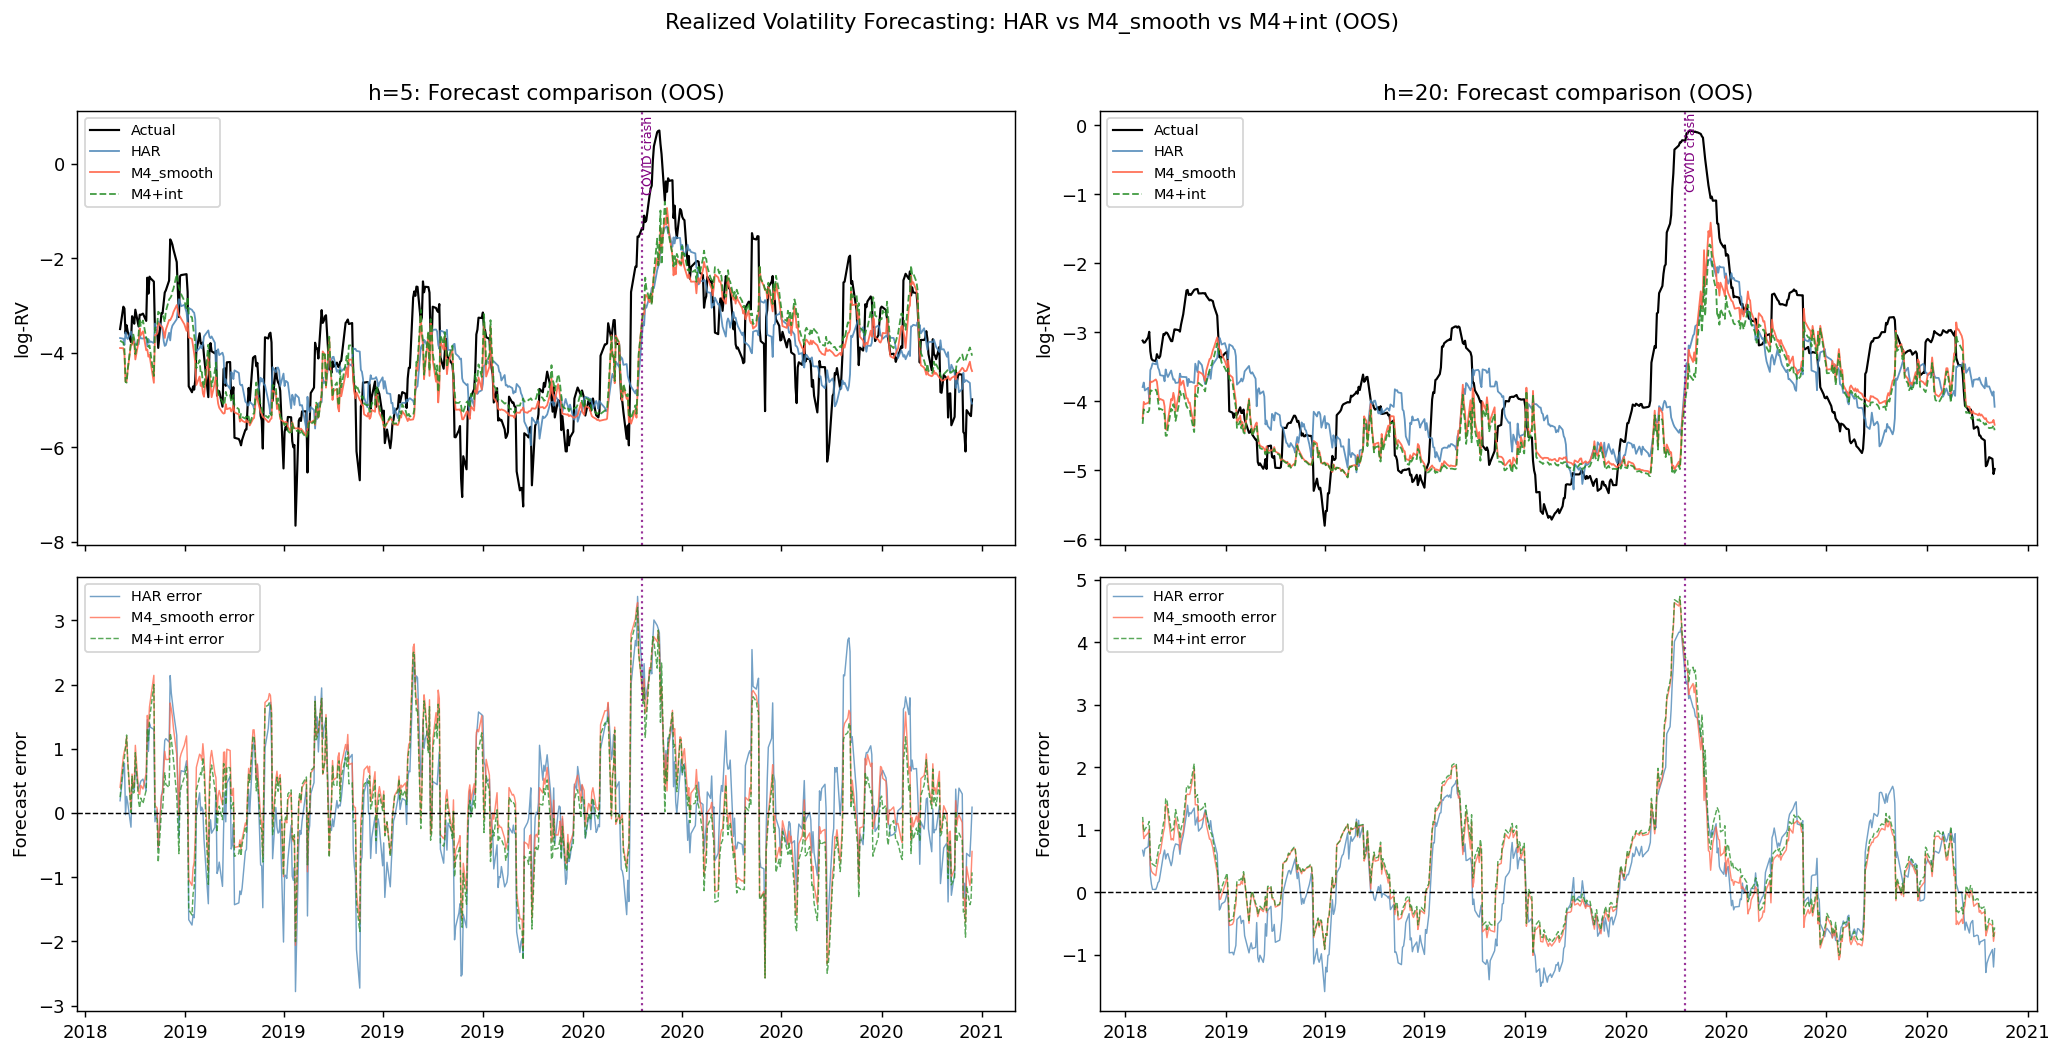
\includegraphics[width=0.82\linewidth,keepaspectratio]{output/figures/C_forecast_comparison.png}
\caption{Out-of-sample realized-volatility forecasts versus realized log-RV through the COVID-19 stress window. Top panels: actual log-RV (black) against the HAR benchmark and the option-augmented M4 specifications at horizons $h=5$ and $h=20$; the vertical marker locates the March-2020 shock (VIX $\approx$ 83). Bottom panels: corresponding forecast errors. The option-implied models track HAR in calm periods but overshoot during the shock, illustrating HAR's parsimony advantage.}
\end{figure}

\textbf{Outcome.} HAR is the best model: every option-augmented specification is statistically \textit{worse} OOS (DM up to -3.59*** at h=5), and even the portable F3\_ATM trails HAR (-2.47** at h=5). In an \textbf{expanding-window} re-evaluation (2016--2020 OOS) all option models converge to HAR performance and HAR+VIX is only nominally best (DM not significant, p $\approx$ 0.26). The richer models overfit the pre-COVID distribution; HAR's parsimony delivers robustness. The honest, well-identified verdict: a single asset's own option surface carries \textbf{no incremental RV-forecasting power beyond HAR} through this stressed window --- the portable approach is viable (F3\_ATM converges to HAR in calm windows) but not superior on this sample.

\begin{figure}[H]\centering
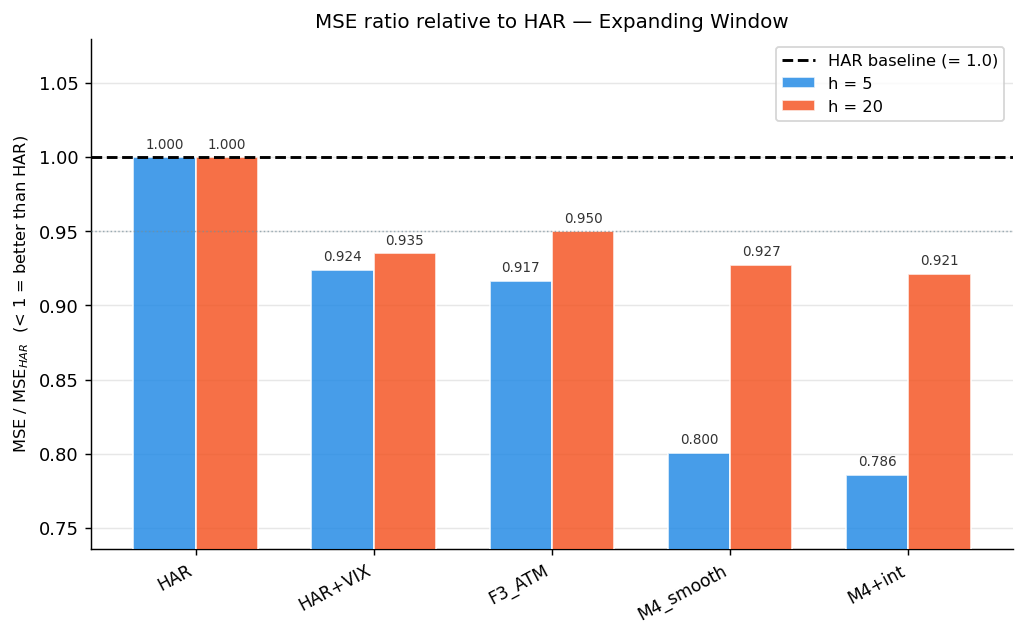
\includegraphics[width=0.82\linewidth,keepaspectratio]{output/figures/C_mse_ratio_bar.png}
\caption{Expanding-window out-of-sample MSE of each forecasting model relative to the HAR benchmark (ratio $<$ 1 $\Rightarrow$ better than HAR), at horizons $h=5$ and $h=20$. Under the expanding-window re-evaluation the option-augmented specifications converge to HAR; only the non-portable HAR+VIX falls nominally below unity, and the gap is not statistically significant. The bars complement the single-split $R^2_\text{OOS}$ of the table above.}
\end{figure}

\textbf{Probabilistic forecasting.} Complementing the point forecasts: AR(1)-GARCH(1,1) (Bollerslev 1986) with QMLE errors produces calibrated \textbf{80\% prediction intervals} for the SSVI parameter paths (Notebook B), and the risk engine below is evaluated by its \textbf{ES\textsubscript{95}} tail coverage (Notebook D).

\subsection*{3.6 Original contributions beyond the core requirements}

The two main extras are the \textit{portable RV-forecasting study} of \S{}3.5 (Notebook C) and the \textit{market-making risk engine} below (Notebook D); two shorter findings follow.

\subsubsection*{(a) A surface market-making risk engine extending Avellaneda-Stoikov --- Notebook D}

We extend the single-instrument optimal market-making model of \textbf{Avellaneda \& Stoikov (2008)} to the \textbf{full implied-volatility surface} (a 45-point grid, 9 strikes $\times$ 5 maturities, 2,633 days). The Avellaneda-Stoikov logic sets a quoting half-spread around a reservation price that scales with the instrument's volatility and the maker's inventory risk; applied surface-wide this gives a vol-scaled baseline spread \texttt{spread\_AS}. The problem is that this baseline systematically \textit{under-covers} the realised next-day surface move (it ignores the part of surface risk not captured by a simple vol scaling), so we add an \textbf{SSVI-based residual-risk add-on} fed by a HAR-J forecast of surface realized volatility, and calibrate it to a target tail (ES\textsubscript{95}) coverage by maturity bucket.

\begin{itemize}\setlength{\itemsep}{1pt}
\item \textbf{Add-on term structure.} The calibrated add-on coefficient follows $c^*(T) = 4.950 - 3.208\sqrt{T}$ (R\textsuperscript{2} = \textbf{0.949}) --- strictly decreasing in maturity, economically sensible: short-dated IV moves are more volatile relative to their long-run expectation and require a larger relative buffer. The $\sqrt{T}$ form is consistent with Brownian surface dynamics.
\item \textbf{Coverage.} The AS baseline alone covers only \textbf{57.3\%} of next-day surface moves globally (19.4\% at 1M, 48.1\% at 3M) --- far below the 95\% target. With the residual-risk add-on (which makes up \textbf{74\%} of the total spread) coverage reaches \textbf{95.9\%} globally (97.4\% 1M, 96.9\% 3M); pointwise surface containment rises from \textbf{47.5\%} to \textbf{82.9\%}.
\item \textbf{Jump robustness.} A bipower-variation jump filter (BPV) flags 29.7\% of days --- too loose --- so a q95+2$\sigma$ threshold (1.4\% jump rate) is selected; the HAR-J jump term does not improve the surface-RV forecast (DM p = 0.290), so jumps are retained only as a robustness check, not a driver.
\item \textbf{Sensitivity.} Varying the baseline tightness $\gamma$ shows a sharp non-linear transition between $\gamma$ = 1.0 and $\gamma$ = 2.0 (where \texttt{c*} collapses $\approx$2.2 $\rightarrow$ $\approx$0.07): once the baseline quote is wide enough the vol-scaled AS spread alone nears the 95\% target and the add-on becomes redundant --- identifying the operating regime in which the SSVI add-on actually adds value.
\end{itemize}

\begin{figure}[H]\centering
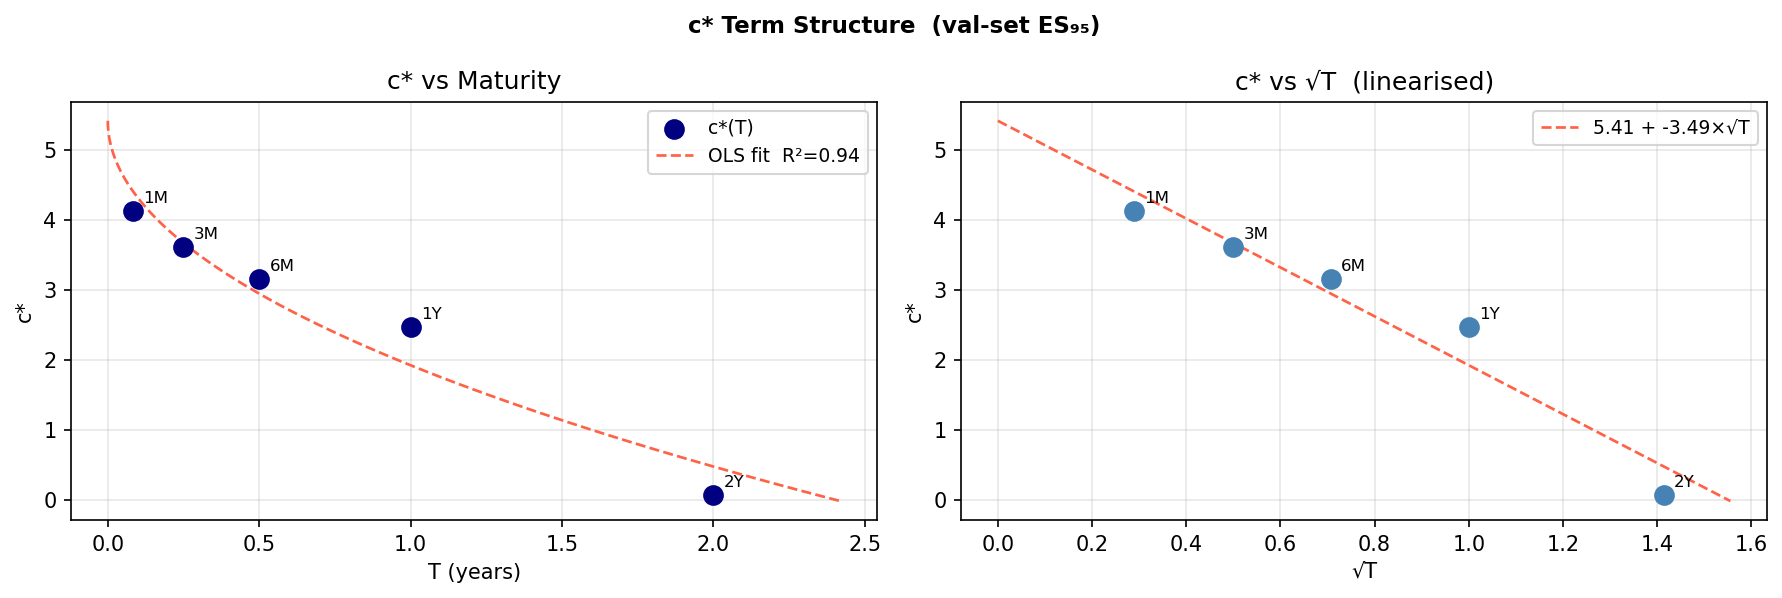
\includegraphics[width=0.82\linewidth,keepaspectratio]{output/plots/D_cstar_term_structure.png}
\caption{Maturity term structure of the calibrated ES\textsubscript{95} residual-risk add-on coefficient $c^*(T)$. Left: $c^*$ against maturity $T$ with the fitted decay; right: the same coefficients against $\sqrt{T}$, linearised as $c^*(T) = 4.95 - 3.21\sqrt{T}$ (R\textsuperscript{2} = 0.95). The monotone decline in maturity is consistent with Brownian surface dynamics --- short-dated implied-variance moves are larger relative to their long-run mean and require a proportionally wider buffer.}
\end{figure}

The engine is \textbf{portable} (it uses only the asset's own calibrated surface) and turns the SSVI model into a deployable quoting-and-risk tool --- the project's most direct operational contribution.

\subsubsection*{(b) Other findings}

\noindent \textbf{HAR on the SSVI parameters: no genuine multi-horizon memory.} A HAR(1,5,22) on the \textit{differenced} parameters posts R\textsuperscript{2}\_OOS = 0.51--0.67 vs. the random walk for all five series. The differenced parameters carry \textit{negative} lag-1 autocorrelation (-0.09 to -0.36, bid-ask-bounce-like mean reversion), so we benchmark HAR against the \textbf{expanding historical mean} (a trivial constant forecast, with a Diebold-Mariano test) and against the ARMA of \S{}3.4 to separate genuine multi-horizon structure from simple shrinkage toward the mean:

\begin{center}\footnotesize
\begin{tabularx}{\textwidth}{l Y Y Y Y Y}
\toprule
\textbf{Series} & \textbf{HAR R\textsuperscript{2}\_OOS (vs RW)} & \textbf{Constant-mean R\textsuperscript{2}\_OOS (vs RW)} & \textbf{HAR R\textsuperscript{2}\_OOS (vs constant-mean)} & \textbf{DM (p)} & \textbf{ARMA MSE-ratio} \\
\midrule
d\_alpha & 0.5664 & 0.5709 & -0.0105 & -0.71 (0.48) & 0.4272 \\
d\_beta & 0.5506 & 0.5534 & -0.0064 & -0.42 (0.67) & 0.4445 \\
d\_rho & 0.5092 & 0.5331 & -0.0511 & -0.80 (0.43) & 0.5254 \\
d\_eta & 0.5642 & 0.5700 & -0.0135 & -0.11 (0.91) & 0.4471 \\
d\_gamma & 0.6661 & 0.6223 & \textbf{+0.1162} & +0.64 (0.52) & \textbf{0.3166} \\
\bottomrule
\end{tabularx}
\end{center}

The constant-mean forecast alone reaches R\textsuperscript{2}\_OOS = 0.53--0.62 vs. random walk --- essentially matching HAR for $\alpha$, $\beta$, $\rho$, $\eta$, where HAR adds nothing on top of it.

\textbf{$\gamma$ is the partial exception:} HAR beats the constant mean by +0.12 in R\textsuperscript{2}\_OOS terms, but the DM test cannot distinguish that edge from noise (p = 0.52) and the plain MA(1) of \S{}3.4 (ratio 0.317) matches or beats HAR (0.334) anyway. $\gamma$'s predictability is therefore \textit{one-lag mean-reversion}, consistent with its stronger persistence and structural-break profile (S2 Chow tests, rolling-Johansen), not multi-horizon memory.

The Andr\`{e}s et al. (2025)-inspired hypothesis --- that the parameters' own multi-horizon history forecasts their future innovations --- thus finds no support beyond short-memory dynamics, consistent with the efficiently-priced, near-martingale surface documented throughout this section.

\noindent \textbf{PCA / regimes (brief).} PCA on surface \textit{changes} gives PC1 = 92.7\% (common shift), and a HAR on the PC scores returns negative R\textsuperscript{2}\_OOS (-0.004/-0.020/-0.008), consistent with the efficient-surface reading. A 3-state HMM on $\Delta$IV identifies low/mid/high-vol regimes (24\%/25\%/50\% of days); supplementary notebook S2 adds Chow break tests (Volmageddon 2018, COVID 2020), CUSUM stability and Granger-causality checks.

\subsection*{3.7 Limitations and robustness}

1. \textbf{Distributional shift.} The 2018--2020 test window contains COVID-19, an extreme OOS regime; the negative option-feature results should be re-checked on a calmer window (e.g. 2015--2018).

2. \textbf{Single underlying / single SSVI variant.} Results are specific to SPX and to the power-law $\phi$($\theta$); raw SVI, eSSVI or SABR could differ.

3. \textbf{VECM / cointegration instability.} Rolling Johansen shows the rank is regime-conditional; the VECM's OOS failure may reflect structural breaks rather than absence of a relationship.

4. \textbf{Expanding-window convergence.} Option-augmented models converge to HAR in the expanding window, so part of the single-split deficit is small-sample, not structural.

\section*{4. Conclusion}

The project's central empirical result is \textbf{negative with informational content}: a structurally rich, arbitrage-free SSVI surface does \textit{not} improve on a parsimonious HAR for realized-volatility forecasting, and at the daily frequency the surface behaves like a near-efficiently-priced, near-martingale object (\S{}3.4--\S{}3.6). This answers our first research aim: replacing the SPX-specific VIX with portable, option-implied regime features is \textit{viable but not superior} on this sample --- the leading portable model (F3\_ATM) converges to HAR in calm windows but cannot beat it through the COVID-19 shock. That HAR wins is itself the economically meaningful finding: backward-looking long-memory structure, not forward-looking surface geometry, carries short-horizon RV predictability here.

The second aim delivers the main operational contribution: extending \textbf{Avellaneda \& Stoikov (2008)} to the full implied-volatility surface, an SSVI-based residual-risk add-on with a $\sqrt{T}$-calibrated term structure (R\textsuperscript{2} = 0.949) raises ES\textsubscript{95} coverage to \textbf{95.9\%} --- a portable, deployable quoting-and-risk tool using only the asset's own options. Three supporting results frame these contributions: a fully arbitrage-free SSVI calibration database (2,633 daily surfaces, 95.1\% success); a panel decomposition in which moneyness, maturity and day effects explain 86\% of IV cross-sectional variation (96\% with Surface-Cell FE) --- SSVI supplies shape, not signal; and a single narrow predictability result, the wing-decay parameter $\gamma$, whose modest mean-reversion is fully captured by a plain MA(1). Every core econometric technique is exercised on the data, and the two extensions embed the standard toolbox in a genuine quantitative-finance application.

\section*{5. Bibliography}

\begin{itemize}\setlength{\itemsep}{1pt}
\item Andersen, T., Bollerslev, T., Diebold, F. \& Labys, P. (2003). Modeling and forecasting realized volatility. \textit{Econometrica}, 71(2), 579--625.
\item Andr\`{e}s, H., Boumezoued, A. \& Jourdain, B. (2025). The implied volatility surface (also) is path-dependent. \textit{arXiv preprint}.
\item Avellaneda, M. \& Stoikov, S. (2008). High-frequency trading in a limit order book. \textit{Quantitative Finance}, 8(3), 217--224.
\item Bollerslev, T. (1986). Generalized autoregressive conditional heteroskedasticity. \textit{Journal of Econometrics}, 31(3), 307--327.
\item Corsi, F. (2009). A simple approximate long-memory model of realized volatility. \textit{Journal of Financial Econometrics}, 7(2), 174--196.
\item Diebold, F. \& Mariano, R. (1995). Comparing predictive accuracy. \textit{Journal of Business \& Economic Statistics}, 13(3), 253--263.
\item Engle, R. \& Granger, C. (1987). Co-integration and error correction: representation, estimation, and testing. \textit{Econometrica}, 55(2), 251--276.
\item Gatheral, J. \& Jacquier, A. (2014). Arbitrage-free SVI volatility surfaces. \textit{Quantitative Finance}, 14(1), 59--71.
\item Johansen, S. (1991). Estimation and hypothesis testing of cointegration vectors in Gaussian vector autoregressive models. \textit{Econometrica}, 59(6), 1551--1580.
\end{itemize}

\end{document}
